\subsubsection{Admin}
  The final user of CPP: Connect is the department admins, for this example we will describe a journey our supervisor, William Knottenbelt, might take through the system.
  \paragraph{Sign up:}
    Since the software is primarily for the Department of Computing, with other departments being given access at a later date. We have kept initial department creation to be asked for to the database maintainer. 
    Therefore our system in it's earliest stages will be handed over to the Deparment of Computing with William Knottenbelt as the initial supervisor. 

  \paragraph{Dashboard:}
    On signing in Will is directed to his dashboard, where he can then easily add other department admins, such as Sernea Coltress, the Department of Computing's Industrial Liaison Officer in order to balance the work load of the site. This is very much like a company administrators new administrator process.

    % TODO: DASH PICTURE ONCE EMAIL STUFF IS IN

    Will also has the option to set company notifications which will be shown whenever a company tries to create a new event or placement. For example he can add URLs to health and saftey placement forms etc. that must be filled out in order for industrial placements to be approved by the college. 

    Will then notices his approvals section, here he must approve Amazon's emails that have been sent and by viewing the directly send email list he takes mental note that they have invited Jack to interview. 

    %TOOD: Don't have XXX pick a company for print screens
    He also can approve new companies permissions to access his departments students or just to advertise events and placements. Here he deems XXX acceptable since they too are a Corporate Partner.

  \paragraph{Students:}
    Next Will has been asked by a current student, Sarah Tattersall, to sign her up. Although she should be expected to sign herself up, to reduce the work load for Will, he decides this once just to allow it.
    He first navigates to the students list, via his navigation bar and then clicks on the `New Student' button.
    On signing Sarah up he is then taken to the student edit page which is slightly different to what students see so that it is very easy for Will to sign a student up.

    \begin{figure}[H]\centering
    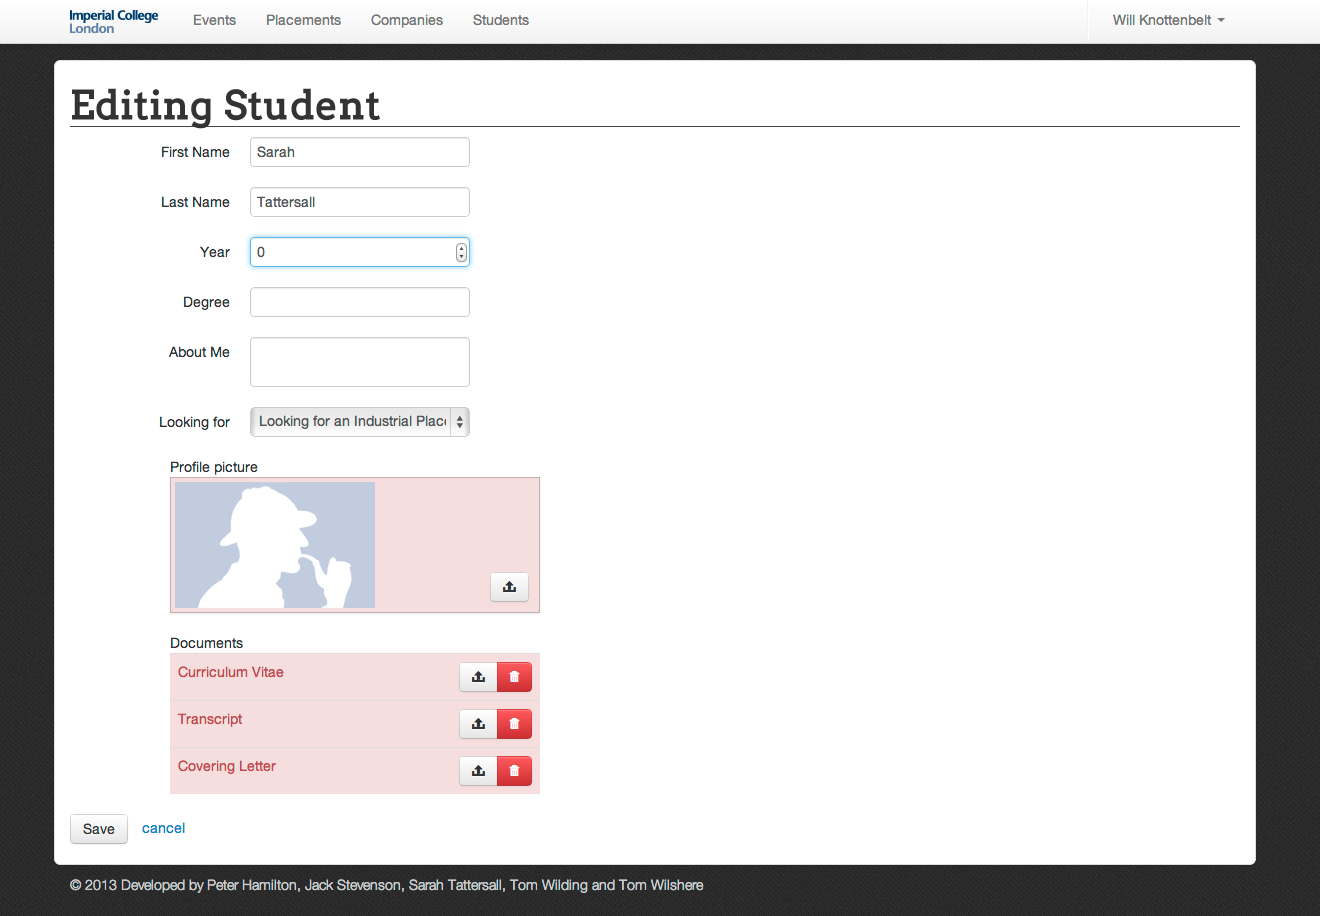
\includegraphics[scale=0.3]{images/user_experiences/admin/admin_student_edit}
    \caption{Student edit page for department administrators}
    \end{figure}

    On clicking save he is taken to her student view. 

    Will also has the right to be able to delete any students who have either left the department or are causing a problem on the site. We hope the latter will not happen but it is a risk that could arrise when students are allowed to develop their own profile.

  \paragraph{Companies:}
    Will can edit, create, and delete companies in exactly the same way as students and can also be directed to a page the edits the companies contacts directly. 

    \begin{figure}[H]\centering
    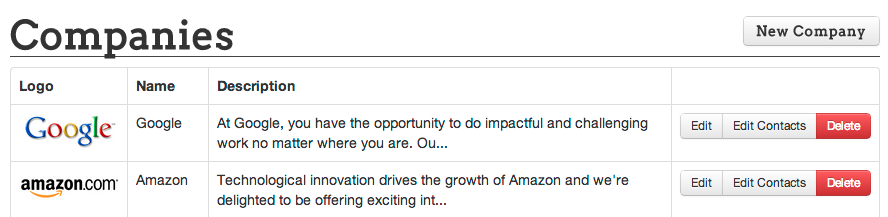
\includegraphics[scale=0.5]{images/user_experiences/admin/admin_company_edit_options}
    \caption{Department admin company edit options}
    \end{figure}

  \paragraph{Emails:}
    Much like companies Will may wish to send an email out to the department students. Instead of using the Imperial email system, he chooses to send it on here because the tagging system allows smart elimination of students who do not want to receive these sort of emails, thus reducing the number of complaints he receives! Will chooses to send an email out detailing some interesting competitions students can get involved in. Since he's a department administrator he does not have to receive approval for these and they are sent straight away.

    If Will decides he wants to know what personal emails are being sent he can view these via the link ...[WHERE IS IT IM NOT SURE IF ITS IMPLEMENTED AT THE TIME OF WRITING]. Being able to view direct emails gives Will the knowledge of what companies are contacting students and how often the site is really being used. This was a big gripe about the previous system since Will had no way of knowing if companies were indeed contacting students.
